\documentclass[aspectratio=169]{beamer}

\usepackage{amsmath,amssymb,amsfonts,amsthm}
\usepackage[T1]{fontenc}
\usepackage[utf8]{inputenc}
\usepackage[english]{babel}
\usepackage{hyperref}
\usepackage{lmodern}
\usepackage{comment}
\usepackage{xcolor}
\usepackage{graphicx,subcaption}
\usepackage[linesnumbered,ruled,vlined,noend,algo2e]{algorithm2e}
\usepackage{tcolorbox}

\renewcommand{\epsilon}{\varepsilon}
\newcommand{\R}{\mathbb{R}}
\newcommand{\N}{\mathbb{N}}
\newcommand{\B}[2]{\mathcal{B}_{#1}\left(#2\right)}
\newcommand{\todo}[1]{{\color{red}#1}}

% Use Unipd as theme, with options:
% - pageofpages: define the separation symbol of the footer page of pages (e.g.: of, di, /, default: of)
% - logo: position another logo near the Unipd logo in the title page (e.g. department logo), passing the second logo path as option 
% Use the environment lastframe to add the endframe text
\usetheme[pageofpages=of]{Unipd}
\usefonttheme[onlymath]{serif}

\title{Random subsampling techniques for sea bass mortality prediction}
\author{Giovanni Gaio, Simone Moretti}
\date{\today}
\subtitle{}

\date{\today}

% The next block of commands puts the table of contents at the beginning of each section and highlights the current section

\begin{comment}
\AtBeginSection[]
{
  \begin{frame}
    \frametitle{Table of Contents}
    \tableofcontents[currentsection]
  \end{frame}
}
\end{comment}


\begin{document}

\frame{\titlepage}

\begin{frame}{Agenda}
    \tableofcontents
\end{frame}

\section{Introduction}
\begin{frame}{Introduction}
\end{frame}

\begin{frame}{Methodology: subsampling}
\end{frame}

\section{Results}
\begin{frame}{Results}
\end{frame}

\begin{frame}{Results: uniform subsampling}
\begin{figure}[ht!]
    \centering
    \begin{subfigure}[t]{0.49\textwidth}
    \centering
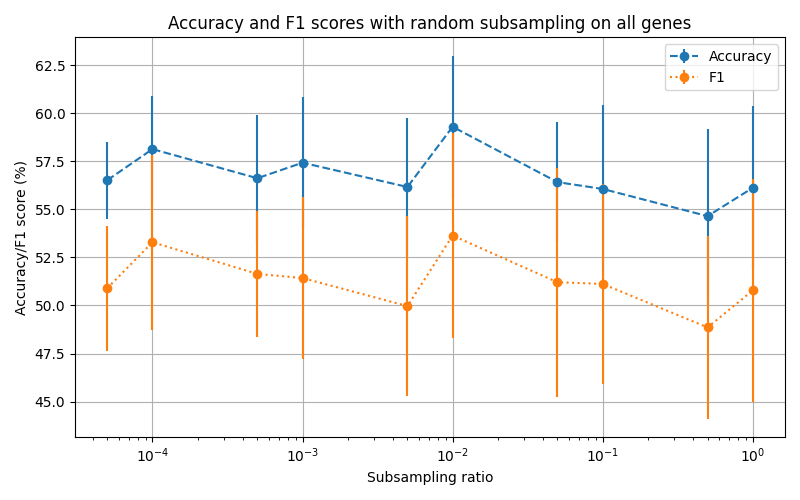
\includegraphics[width=\columnwidth]{../figures/subsample_plot.png}
\caption{Plot of the scores when subsampling uniformly on the whole genome.}
\label{fig:res1a}
    \end{subfigure}
    \begin{subfigure}[t]{0.49\textwidth}
    \centering
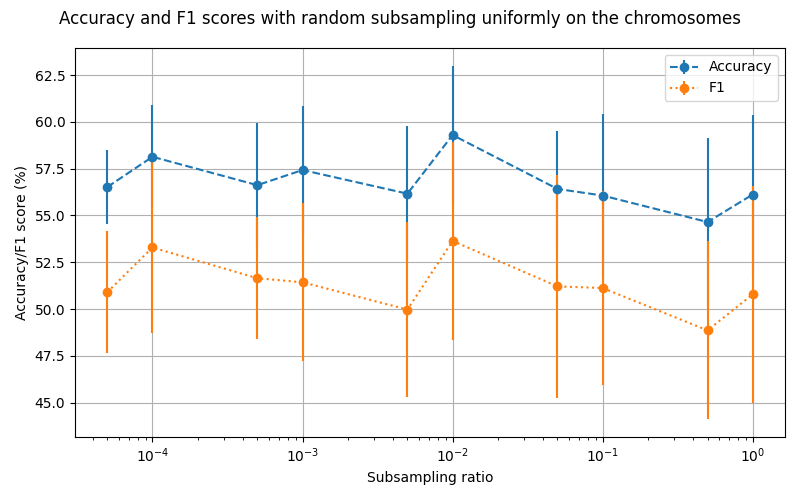
\includegraphics[width=\columnwidth]{../figures/uniform_sample_low_ratio.png}
\caption{Plot of the scores when subsampling uniformly on each chromosome.}
\label{fig:res1b}
    \end{subfigure}
\caption{Plots of accuracy and F1 scores for different subsampling rates on the whole genome.}
\label{fig:res1}
\end{figure}
\end{frame}

\begin{frame}{Results: annotated subsampling}
\begin{figure}[ht!]
\centering
\begin{subfigure}[ht]{\textwidth}
    \centering
    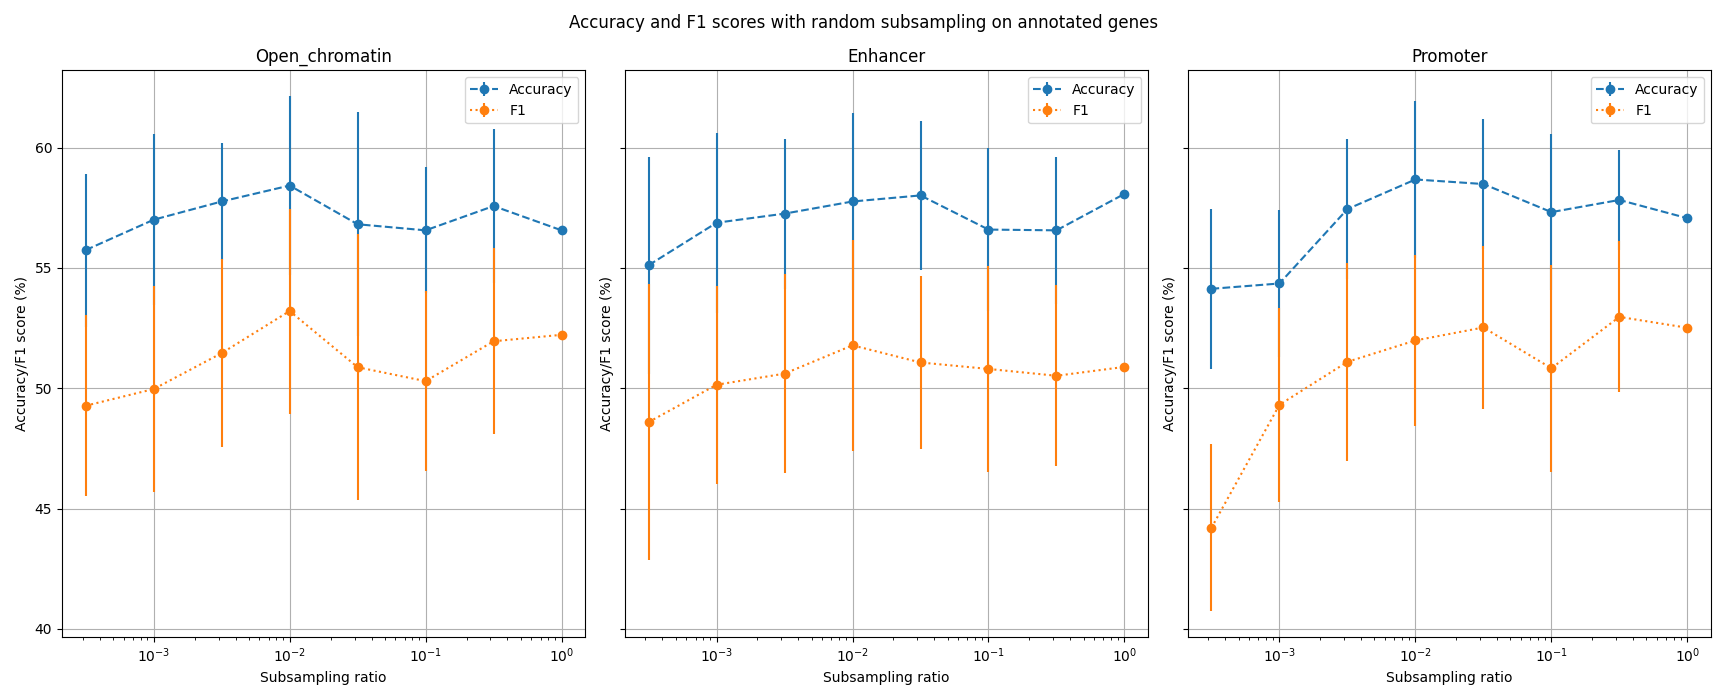
\includegraphics[width=\textwidth]{../figures/subsample_annotated.png}
\caption{Plots of the scores while subsampling genes annotated in different categories.}
\label{fig:res2a}
\end{subfigure}

\begin{subfigure}[ht]{\textwidth}
\centering
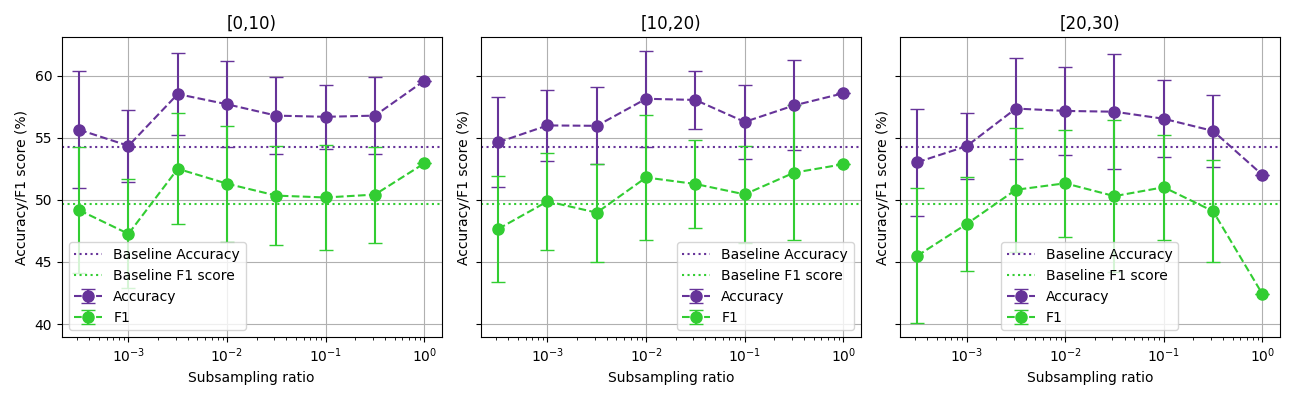
\includegraphics[width=\textwidth]{../figures/subsample_ntissue.png}
\caption{Plots of the scores while using only genes with tissue number in a given range.}
\label{fig:res2b}
\end{subfigure}
\caption{Plots of the accuracy and F1 scores for the different subsampling rates on the annotated genes. Each single plot is done using only the genes annotated with the indicated values.}
\label{fig:res2}
\end{figure}
\end{frame}

\section{Conclusions}
\begin{frame}{Conclusions}
\end{frame}

\end{document}

